%%!TEX encoding = UTF-8 Unicode

% Several lines in file have comments suggesting common packages for the
% typical thesis in informatics or electronics developed at UA
% uncomment/comment the lines as required for your work
% Before each optional line you will have a small comment

% According to UA rules, font size should range from 10 to 12pt.
\documentclass[11pt,a4paper,oneside,onecolumn]{memoir}

\listfiles
\fixpdflayout

\usepackage[utf8]{inputenc}

% Select Computer Modern Typewritter (For bold ttfamily in listings)
\usepackage{lmodern}
% OR... Bera Mono
%\usepackage[scaled]{beramono} % TTT Font
%\usepackage{anyfontsize} % As the name says...

\usepackage[T1]{fontenc}

% Enable for for Overleaf support
\usepackage{ifthen}
\def\useoverleaf{0}  % change to non-zero (for instance, 1) to enable it

\makeatletter
\newcommand{\makecoverfile}[0]{%
  \immediate\write18{latexmk -pdf cover.tex}%
}
\makeatother

% For PDF merging
\usepackage{pdfpages}

% Set DPI to 300
\pdfpxdimen=\dimexpr 1in/300\relax

% Allow the use of a larger number of packages
\usepackage{morewrites} 

% For English and Portuguese languages
% Portuguese will be the default.
% Uncomment \setlanguage below to change it
\usepackage[english,portuguese]{babel}

% Uncomment to use a custom date format
%\usepackage{datetime}
%\newdateformat{thesisdate}{\monthname[\THEMONTH] \THEYEAR} % Month Year

% Make pdf look better
\usepackage{microtype} 

% Uncomment to enable floats on facing pages
%\usepackage{dpfloat}

% Side by side figures
% Eg. Fig 1a, Fig 1b
\usepackage[hang,small,bf]{caption}
%\let\tion\undefined
%\let\subfloat\undefined
\usepackage{subcaption}

%\RequirePackage{textcase}

% Dropped Caps
%\usepackage{lettrine}

% Configure Hyperlink color
% As a matter or style, you may use this to enable/disable color boxes on links
%\usepackage[breaklinks=true,colorlinks=false,linkcolor=blue]{hyperref}
% Or use the default values provided by the hyperref package
\usepackage{hyperref}

% Redefine section names according to your preference
%\def\sectionautorefname{Section}
%\def\chapterautorefname{Chapter}
%\def\figureautorefname{Figure}
%\def\listingautorefname{Listing}
%\def\tableautorefname{Table}

% Redefine code boxes
\ifthenelse{\equal{\useoverleaf}{0}}
{\usepackage[outputdir=build]{minted}}
{\usepackage{minted}}%

\addto\captionsportuguese{%
  \renewcommand\listingscaption{Código}
}
\fvset{fontsize=\footnotesize} % Make Code blocks smaller than text
\usepackage{csquotes}

% Add support for PDF Comments
\usepackage{comment}
\ifthenelse{\equal{\useoverleaf}{0}}
{\usepackage{pdfcomment}}{}
\usepackage{bookmark} % New Bookmarks

% For Multiple columns in Glossary
\usepackage{multicol}

% Add support for Math symbols
\usepackage{amsmath}
\usepackage{amssymb}

% Add support for graphics
\usepackage{graphicx}

% Add support for Colors
\usepackage{xcolor}

% Add support for the Euro symbol
\usepackage{eurosym}

% Add support for missingfigure and todo
\usepackage{todonotes}

% Setup bibliography with Biber using IEEE style for proper UTF-8 support
\usepackage[backend=biber, style=ieee, sorting=none, natbib=true, mincitenames=1, maxcitenames=2]{biblatex}
\bibliography{bib/references.bib}

% Use acronyms
\usepackage[printonlyused]{acronym} % For acronyms

% Indenting the first paragraph after section start
\usepackage{indentfirst}

% For fixing listoflistings with memoir
\usepackage{xparse}

% Uncomment the next lines to enable chart support through pgf and tikz
% This may require you to install further packages in your Tex system
%\usepackage[version=0.96]{pgf}
%\usepackage{tikz}

% UML support
%\usepackage{pgf-umlsd}

% Trees, Arrows, Mindmaps and other popular objects
%\usetikzlibrary{arrows,shadows,trees,shapes,decorations,automata,backgrounds,petri,mindmap} % for pgf-umlsd

% Package to master SI units
\usepackage[detect-weight=true, binary-units=true]{siunitx}
% For Electric Circuits
%\sisetup{load-configurations = binary}

% Set Voltage direction accordingly
% Option : oldvoltagedirection,nooldvoltagedirection,RPvoltages,EFvoltages
% More information at: https://mirrors.ibiblio.org/CTAN/graphics/pgf/contrib/circuitikz/doc/circuitikzmanual.pdf
% By default this template is using the Old Voltage Direction
%\usepackage[oldvoltagedirection,american,cuteinductors,smartlabels]{circuitikz}
%\usetikzlibrary{calc}
%\ctikzset{bipoles/thickness=1}
%\ctikzset{bipoles/length=0.8cm}
%\ctikzset{bipoles/diode/height=.375}
%\ctikzset{bipoles/diode/width=.3}
%\ctikzset{tripoles/thyristor/height=.8}
%\ctikzset{tripoles/thyristor/width=1}
%\ctikzset{bipoles/vsourceam/height/.initial=.7}
%\ctikzset{bipoles/vsourceam/width/.initial=.7}
%\tikzstyle{every node}=[font=\small]
%\tikzstyle{every path}=[line width=0.8pt,line cap=round,line join=round]

% For inline TT text (e.g. code snippets)
\usepackage{verbatim}

% Frames around figures and allow force placement
\usepackage{float}

% Configure Float style
%\floatstyle{boxed}
%\restylefloat{table}
%\restylefloat{figure}
%\restylefloat{lstlisting}

% For test purposes you may use the lipsum package to create dummy text
\usepackage{lipsum} % REMOVE

%Keep floats inside section!
\usepackage[section]{placeins}
\let \oldsubsubsection \subsubsection
\renewcommand{\subsubsection}[2][]{
  \FloatBarrier
  \oldsubsubsection#1{#2}
}
\let \oldsubsection \subsection
\renewcommand{\subsection}[2][]{
  \FloatBarrier
  \oldsubsection#1{#2}
}
\let \oldsection \section
\renewcommand{\section}[2][]{
  \FloatBarrier
  \oldsection#1{#2}
}
\let \oldchapter \chapter
\renewcommand{\chapter}[2][]{
  \FloatBarrier
  \oldchapter#1{#2}
}



% Use the built-in division styling
\headstyles{memman}

% Include subsections in the TOC
\settocdepth{subsection}

% Numbering down to subsections as well
\setsecnumdepth{subsection}

% extra index for first lines
\makeindex[lines]

% Margins for University of Aveiro Thesis
\setlrmarginsandblock{3cm}{2.5cm}{*}
\setulmarginsandblock{3cm}{3cm}{*}
\checkandfixthelayout

% Or select your custom spacing to make any ajustment
%\addtolength{\parskip}{0.5\baselineskip}
\linespread{1.5}

\newcommand\mainmatterWithoutReset
{\edef\temppagenumber{\arabic{page}}%
  \mainmatter
  \setcounter{page}{\temppagenumber}%
}


%%%%%%%%%%%%%%%%%%%%%%%%%%%%%%%%%%%%%%%%%%%%%%%%%%
% Document begins here
%%%%%%%%%%%%%%%%%%%%%%%%%%%%%%%%%%%%%%%%%%%%%%%%%%

\begin{document}

% Fix the numbering scheme by having a ghost style for page numbering
\pagenumbering{Alph}

\ifthenelse{\equal{\useoverleaf}{0}}{}{\makecoverfile{}}%
\setcounter{page}{0}
\includepdf[pages=-]{cover.pdf}

% Uncomment to enable English
\selectlanguage{english}


% Front matter

%Custom Chapter style named `thesis`
\makechapterstyle{thesis}{% Based on ell
  \chapterstyle{default}
  \renewcommand*{\chapnumfont}{\normalfont\sffamily}
  \renewcommand*{\chaptitlefont}{\normalfont\Huge\sffamily}
  \settowidth{\chapindent}{\chapnumfont 111}
  \renewcommand*{\chapterheadstart}{\begingroup
    \vspace*{\beforechapskip}%
    \begin{adjustwidth}{}{-\chapindent}%
      \hrulefill
      \smash{\rule{0.4pt}{15mm}}
    \end{adjustwidth}\endgroup}
  \renewcommand*{\printchaptername}{}
  \renewcommand*{\chapternamenum}{}
  \renewcommand*{\printchapternum}{%
    \begin{adjustwidth}{}{-\chapindent}
      \hfill
      \raisebox{10mm}[0pt][0pt]{\fontsize{30}{25}\selectfont\chapnumfont \thechapter}%
      \hspace*{1em}
    \end{adjustwidth}\vspace*{-3.0\onelineskip}}
  \renewcommand*{\printchaptertitle}[1]{%
    \vskip\onelineskip
    \raggedleft {\chaptitlefont ##1}\par\nobreak\vskip 4\onelineskip}}


% Select chapter style from existing or select custom
%\chapterstyle{thesis} % Others: dowding, demo2, dash, chappell, brotherton, bianchi, ger, madsen, tatcher, veelo,indexes)
% thesis can also be used as defined previously
% Check the memoir documentation for the available themes
% Default is veelo
\chapterstyle{veelo}
\makeoddfoot{plain}{}{\thepage}{} % Added by André Zúquete to fix a page numbering issue on the veelo chapter style

% Select Page style
\pagestyle{plain}

% If you feel adventurous you can also define all aspects of your theme
% Use either this input or the chapterstyle before
% % Rules
\newcommand{\thinRule}{\rule{\textwidth}{0.25pt}}

% Customize heading appearances
% Define styles
\newcommand{\partSize}{\Huge}
\newcommand{\partStyle}{\lsstyle\scshape}
\newcommand{\chapterSize}{\Huge}
\newcommand{\chapterStyle}{\lsstyle\scshape}
\newcommand{\chapterAfter}{}
\newcommand{\sectionSize}{\Large}
\newcommand{\sectionStyle}{\scshape\MakeTextLowercase}
\newcommand{\subsectionSize}{\large}
\newcommand{\subsectionStyle}{\scshape\MakeTextLowercase}
\newcommand{\subsubsectionSize}{\large}
\newcommand{\subsubsectionStyle}{\scshape\MakeTextLowercase}
\newlength{\partNumSizePt}
\setlength{\partNumSizePt}{60pt}
\newlength{\chapterNumSizePt}
\setlength{\chapterNumSizePt}{60pt}
\newcommand{\partNumSize}{%
  \fontsize{\partNumSizePt}{1.2\partNumSizePt}\selectfont%
}
\newcommand{\partNumStyle}{\partChapterNumColor}
\newcommand{\chapterNumSize}{%
  \fontsize{\chapterNumSizePt}{1.2\chapterNumSizePt}\selectfont%
}
\newcommand{\chapterNumStyle}{\partChapterNumColor}

% Customize parts
\renewcommand{\partnamefont}{\partSize\partStyle}
\renewcommand{\partnumfont}{\partNumSize\partNumStyle}
\renewcommand{\printpartname}{}
\renewcommand{\printparttitle}[1]{%
  \normalfont\normalcolor\partnamefont #1
}

% Customize chapters
\makeatletter
\setlength{\beforechapskip}{30pt}
\renewcommand*{\chapterheadstart}{\vspace*{\beforechapskip}}
\setlength{\afterchapskip}{3ex}
\setlength{\midchapskip}{3ex}
\renewcommand*{\chapnamefont}{%
  \Large\flushright\chapterStyle\partChapterNumColor%
}
\renewcommand*{\chapnumfont}{\chapterNumSize\chapterNumStyle}
\renewcommand*{\chaptitlefont}{%
  \normalfont\flushleft\normalcolor\chapterSize\chapterStyle%
}
\renewcommand*{\printchaptername}{%
  \chapnamefont\MakeTextLowercase{\@chapapp}%
}
\renewcommand*{\chapternamenum}{\quad}
\renewcommand*{\printchapternum}{%
%  \chapnumfont\textls[-75]{\classicstylenums{\thechapter}}%
 \chapnumfont\textls[-75]{\thechapter}%

}
\renewcommand*{\printchaptertitle}[1]{%
  \chaptitlefont #1
  \chapterAfter
}
\makeatother
% Customize sections and subsections
\setsecnumformat{\csname my#1\endcsname\quad}
\setsecheadstyle{\sectionSize\sectionStyle}
\newcommand{\mysection}{{\thesection}}
\setlength{\beforesecskip}{3em}


\setsubsecheadstyle{\subsectionSize\subsectionStyle}
\newcommand{\mysubsection}{{\normalfont\subsectionSize\thesubsection}}
\setlength{\beforesubsecskip}{3em}

\setsubsubsecheadstyle{\subsubsectionSize\subsubsectionStyle}
\newcommand{\mysubsubsection}{{\normalfont\subsubsectionSize\thesubsubsection}}
\setlength{\beforesubsubsecskip}{2em}

% Customize "Table of ..." appearance
% Customize headings
\newcommand{\renewPrintXTitle}[1]{%
  \renewcommand{#1}[1]{%
    \printchaptertitle{##1}%
  }%
}
\renewPrintXTitle{\printtoctitle}
\renewPrintXTitle{\printlottitle}
\renewPrintXTitle{\printloftitle}

% Customize ToC headings
\renewcommand{\cftpartfont}{\partChapterNumColor\partStyle}
\renewcommand{\cftchapterfont}{\chapterStyle}
\renewcommand{\cftsectionfont}{}
\renewcommand{\cftsubsectionfont}{}
\renewcommand{\cftfigurefont}{}
\renewcommand{\cfttablefont}{}
\newcommand{\cftlstlistingfont}{}

% Increase number width
\newlength{\cftNumWidthIncrease}
\setlength{\cftNumWidthIncrease}{0.25em}
\addtolength{\cftpartnumwidth}{\cftNumWidthIncrease}
\addtolength{\cftchapternumwidth}{\cftNumWidthIncrease}
\addtolength{\cftsectionindent}{\cftNumWidthIncrease}
\addtolength{\cftsubsectionindent}{\cftNumWidthIncrease}
% No leader dots
%\renewcommand*{\cftpartdotsep}{\cftnodots}
%\renewcommand*{\cftchapterdotsep}{\cftnodots}
%\renewcommand*{\cftsectiondotsep}{\cftnodots}
%\renewcommand*{\cftsubsectiondotsep}{\cftnodots}
%\renewcommand*{\cftfiguredotsep}{\cftnodots}
%\renewcommand*{\cfttabledotsep}{\cftnodots}
%\newcommand*{\cftlstlistingdotsep}{\cftnodots}
% Set page numbers immediately after entry text
\newcommand{\tocEntryPageSep}{\hspace{1em}}
\renewcommand{\cftpartleader}{\cftdotfill{\cftdotsep}}
%\renewcommand{\cftpartafterpnum}{\cftparfillskip}
%\renewcommand{\cftchapterleader}{\tocEntryPageSep}
\renewcommand{\cftchapterleader}{\cftdotfill{\cftdotsep}}
%\renewcommand{\cftchapterafterpnum}{\cftparfillskip}
\renewcommand{\cftsectionleader}{\cftdotfill{\cftdotsep}}
%\renewcommand{\cftsectionafterpnum}{\cftparfillskip}
\renewcommand{\cftsubsectionleader}{\cftdotfill{\cftdotsep}}
%\renewcommand{\cftsubsectionafterpnum}{\cftparfillskip}
\renewcommand{\cftfigureleader}{\cftdotfill{\cftdotsep}}
%\renewcommand{\cftfigureafterpnum}{\cftparfillskip}
\renewcommand{\cfttableleader}{\cftdotfill{\cftdotsep}}
%\renewcommand{\cfttableafterpnum}{\cftparfillskip}
\newcommand{\cftlstlistingleader}{\cftdotfill{\cftdotsep}}
%\newcommand{\cftlstlistingafterpnum}{\cftparfillskip}
% Customize page numbers
\newcommand{\tocPageStyle}{\tocPageColor}
\renewcommand{\cftpartpagefont}{\tocPageStyle}
\renewcommand{\cftchapterpagefont}{\tocPageStyle}
\renewcommand{\cftsectionpagefont}{\tocPageStyle}
\renewcommand{\cftsubsectionpagefont}{\tocPageStyle}
\renewcommand{\cftfigurepagefont}{\tocPageStyle}
\renewcommand{\cfttablepagefont}{\tocPageStyle}
\newcommand{\cftlstlistingpagefont}{\tocPageStyle}

% Abstract
% Remove indents around abstract text
\setlength{\absleftindent}{0pt}
\setlength{\absrightindent}{0pt}
% Change font size to conform with the rest of the document text
\renewcommand{\abstracttextfont}{\normalsize}

% Customize headers and footers including page numbers
\newcommand{\hfTextSize}{\footnotesize}
\newcommand{\headTextStyle}{\lsstyle\scshape\MakeTextLowercase}
\nouppercaseheads
\makeevenhead{headings}%
             {\hfTextSize\thepage}%
             {}%
             {\hfTextSize\headTextStyle\leftmark}
\makeevenhead{plain}%
             {\hfTextSize\thepage}%
             {}%
             {\hfTextSize\headTextStyle\leftmark}
\makeoddhead{headings}%
            {\hfTextSize\headTextStyle\rightmark}%
            {}%
            {\hfTextSize\thepage}
\makeoddhead{plain}%
            {\hfTextSize\headTextStyle\rightmark}%
            {}%
            {\hfTextSize\thepage}


% Customize captions
\newcommand{\captionSize}{\small}
\newcommand{\captionStyle}{\scshape}
\newcommand{\captionWidthRatio}{0.9}

\captionnamefont{\captionSize\captionStyle}
\captiontitlefont{\captionSize}
\captiondelim{ -- }
\captiontitlefinal{}
\changecaptionwidth
%\captionwidth{\captionWidthRatio\textwidth}

% Define colors
%\newcommand{\titleColor}{\color[rgb]{0.616, 0.0627, 0.176}}
\newcommand{\titleColor}{\color[rgb]{0,0,0}}

\newcommand{\partChapterNumColor}{\titleColor}
\newcommand{\dropCapColor}{\titleColor}
%\newcommand{\tocPageColor}{\color[rgb]{0.0980, 0.329, 0.651}}

\newcommand{\tocPageColor}{\color[rgb]{0, 0,0}}
\definecolor{shade0}{rgb}{1.0 , 1.0 , 1.0 }
\definecolor{shade1}{rgb}{0.9 , 0.9 , 0.9 }
\definecolor{shade2}{rgb}{0.8 , 0.8 , 0.8 }
\definecolor{shade3}{rgb}{0.65, 0.65, 0.65}
\definecolor{shade4}{rgb}{0.45, 0.45, 0.45}
\definecolor{shade5}{rgb}{0.0 , 0.0 , 0.0 }



%Exclude sub figures from List of Figures
%\captionsetup[subfloat]{list=no}

% Texts
\newenvironment{introduction}
{%
  \begin{minipage}{\textwidth}%
    \itshape%
    }
    {%
  \end{minipage}%
  \par\addvspace{2\baselineskip plus 0.2\baselineskip minus 0.2\baselineskip}%
}

\frontmatter

\tightlists
\midsloppy
\raggedbottom

\setcounter{tocdepth}{2} %subsections are added to the TOC
\setcounter{secnumdepth}{4} %subsubsections are numbered

% Initial document tables start here: TOC, LOF, LOT, Glossary
% Table of contents with slightly smaller font
{\small\tableofcontents}

% List of figures with slightly smaller font
\clearpage
{\small\listoffigures}

% List of tables with slightly smaller font
\clearpage
{\small\listoftables}

% List of code snippets

% Fix for Listings with memoir

\RenewDocumentCommand \chapter { s O{#3} m }{%
  \FloatBarrier
  \IfValueTF{#1}  % if optional star is seen
  {\oldchapter*{#2}}
  {\oldchapter#1{#2}}
 }

\renewcommand{\listingscaption}{Code}
\renewcommand{\listoflistingscaption}{List of Code Snippets}
%\clearpage
%{\small\listoflistings}
%\addcontentsline{toc}{chapter}{\listoflistingscaption}

% Reset Chapters
\renewcommand{\chapter}[2][]{
  \FloatBarrier
  \oldchapter#1{#2}
}

% Print Glossary
\clearpage
{\small\chapter{Glossary}

\footnotesize
\SingleSpacing

\begin{multicols}{2}
\begin{acronym}[AAAAAA]
\acro{3G}[3G]{third-generation}
\acro{3GPP}[3GPP]{3rd Generation Partnership Project}
\acro{4G}[4G]{fourth-generation}
\acro{5G}[5G]{fifth-generation}
\acro{5G-AKA}[5G-AKA]{5G - Authentication and Key Management}
\acro{5GC}[5GC]{5G Core}
\acro{AV}[AV]{Authentication Vector}
\acro{CP}[CP]{Control Plane}
\acro{EAP}[EAP]{Extensible Authentication Protocol}
\acro{EAP-AKA'}[EAP-AKA']{EAP - Authentication and Key Management}
\acro{EAP-TLS}[EAP-TLS]{EAP - Transport Layer Security}
\acro{eMBB}[eMBB]{enhanced mobile broadband}
\acro{eNodeB}[eNodeB]{evolved Node B}
\acro{EPS}[EPS]{Evolved Packet System}
\acro{EPS-AKA}[EPS-AKA]{Evolved Packet System - Authentication and Key Management}
\acro{GUTI}[GUTI]{Globally Unique Temporary Identity}
\acro{HSS}[HSS]{Home Subscriber Server}
\acro{HN}[HN]{Home Network}
\acro{IMSI}[IMSI]{International Mobile Subscriber Identity}
\acro{IP}[IP]{Internet Protocol}
\acro{MAC}[MAC]{medium access control}
\acro{MMe}[MMe]{Mobility Management Entity}
\acro{mMTC}[mMTC]{massive machine-type communications}
\acro{NAI}[NAI]{Network Access Identifier}
\acro{N5GC}[N5GC]{Non-5G-Capable}
\acro{NFV}[NFV]{Network Functions Virtualization}
\acro{NR}[NR]{5G New Radio}
\acro{SBA}[SBA]{Service Based Architecture}
\acro{SDN}[SDN]{Software Defined Network}
\acro{SEAF}[SEAF]{Security Anchor Function}
\acro{SN}[SN]{Serving Network}
\acro{SUCI}[SUCI]{Subscriber Concealed Identifier}
\acro{SUPI}[SUPI]{Subscription Permanent Identifier}
\acro{TSN}[TSN]{time-sensitive networks}
\acro{UE}[UE]{User Equipment}
\acro{UP}[UP]{User Plane}
\acro{uRLLC}[uRLLC]{ultra-reliable low-latency communications}
\acro{USIM}[USIM]{Universal Subscriber Identity Module}
\acro{WBA}[WBA]{Wireless Broadband Alliance}
\end{acronym}
\end{multicols}

}

%%%%%%%%%%%%%%%%%%%%%%%%%%%%%%%%%%%%%%%%%%%%%%%%%%%%%%%
% Main document starts here
%%%%%%%%%%%%%%%%%%%%%%%%%%%%%%%%%%%%%%%%%%%%%%%%%%%%%%%

\mainmatter

% Line spacing: 1.5 pt 
\OnehalfSpacing

%%%%%%%%%%%%%%%%%%%%%%%%%%%%%%%%%%%%%%%%%%%%%%%%%%%%%%%
% Start of Thesis text 
%%%%%%%%%%%%%%%%%%%%%%%%%%%%%%%%%%%%%%%%%%%%%%%%%%%%%%%

% Uncomment to add further chapters
\chapter{Introduction}%
\label{chapter:introduction}

\begin{introduction}
This chapter summarizes the challenges and significance of integrating Wi-Fi-only devices into the 5G core network, highlighting the limitations of current standards and the need for innovative solutions to enable seamless connectivity and authentication.
\end{introduction}

\section{Background and Context}

% Introduce 5G as a significant advancement in wireless technology, highlighting its core features such as higher speeds, lower latency, and support for diverse use cases (e.g., enhanced mobile broadband, massive machine-type communications, ultra-reliable low-latency communications).

In recent years, \ac{5G} wireless technology has revolutionized telecommunications. It offers higher bandwidth, faster speeds, and lower delays, supporting use cases like \ac{eMBB}, \ac{mMTC}, and \ac{uRLLC}.

Additionally, it is transforming private networks, which have traditionally relied on legacy wired or wireless (WLAN) Ethernet. Features like tighter security, higher reliability, and \ac{TSN} are crucial to meeting Industry 4.0 requirements for wireless connectivity. However, how can the industry bridge the gap between existing \ac{N5GC} devices, which current networks rely on, and new \acp{5GC}?

% Briefly describe the Service Based Architecture of 5G, emphasizing the incorporation of Network Functions Virtualization (NFV) and Software Defined Networking (SDN).
% Mention the various access nodes supported by the 5G system, including native 5G-NR and LTE accesses, and non-3GPP interworking functions.

\ac{5G} is not only a revolution in radio network infrastructure but also in the core network. Now based on Service Based Architecture, using \ac{NFV} and \ac{SDN}, it allows it to minimize cost and maximize utilization and elasticity of the infrastructure by seperating the \ac{UP} functions from the \ac{CP} function. This architecture supports various access nodes such as native \ac{NR}, LTE accesses, and non-\ac{3GPP} interworking functions that facilitate connectivity from untrusted WLANs.~\cite{23.501-p41}

% Discuss the importance of integrating Wi-Fi networks with 5G to enhance connectivity options for users and devices.
% Highlight the challenges posed by current standards that do not support Wi-Fi-only devices without USIM in connecting to the 5G Core.

As wireless networks evolve, the convergence of 5G with existing Wi-Fi infrastructures becomes increasingly critical. However, current standards established by the \ac{3GPP} do not adequately address the integration of Wi-Fi-only devices that lack \ac{USIM} capabilities into the \ac{5GC} network.~\cite{wba-04-2021-p59} This limitation is particularly evident in enterprise environments where many devices operate solely on Wi-Fi. To fully realize the potential of  technology, it is essential to develop solutions that enable integration of Wi-Fi-only devices into the \ac{5G} ecosystem. This includes addressing challenges related to authentication mechanisms, device identity, and overall interoperability between different network types.

\section{Problem Statement}

% - Highlight that the current 3GPP standard does not define an architecture to support Wi-Fi-only devices without USIM connecting to the 5G Core.
% - Emphasize the importance of this issue, especially in enterprise deployments where many devices lack USIM capabilities.
% - Mention the Wireless Broadband Alliance (WBA) recommendation for 3GPP to define procedures for supporting Wi-Fi-only UE with non-IMSI based identity and EAP-TLS/EAP-TTLS based authentication.

The current \ac{3GPP} standard lacks an architecture for integrating Wi-Fi-only devices without \ac{USIM} into the \acl{5GC}, creating a significant gap in connectivity. This limitation is problematic in enterprise environments, where many devices operate ony on Wi-Fi and do not possess \ac{USIM} capabilities. The \ac{WBA} has identified this issue, recommending that \ac{3GPP} develop procedures to support Wi-Fi-only \ac{UE} using non-\acs{IMSI} based identity and authentication methods such as \ac{EAP-TLS} or \ac{EAP-TTLS}. Addressing this challenge is crucial for enabling integration of diverse device types into the \ac{5G} ecosystem.

\section{Research Objectives}

% - State your primary goal: to explore and develop solutions for integrating Wi-Fi-only devices without USIM into the 5G Core infrastructure.
% - List specific objectives, such as:
%   - Investigating authentication mechanisms compatible with both 5G and Wi-Fi networks.
%   - Developing a method for device identification that works across 5G and non-3GPP networks.
%   - Proposing extensions or alternatives to existing protocols to support seamless integration.

The main goal of this research is to explore and develop solutions for integrating Wi-Fi-only devices without \ac{USIM} into the \ac{5GC} infrastructure. To achieve this, we have identified the following specific objectives:

\begin{enumerate}
    \item{
        Investigate authentication mechanisms compatible with both \ac{5G} and Wi-Fi networks:
        \begin{itemize}
            \item Analyze existing authentication methods such as \ac{EAP-TLS} and \ac{EAP-TTLS} for their applicability in a converged \ac{5G}-Wi-Fi environment.
            \item Explore potential modifications or extensions to these methods to ensure seamless authentication across different network types.
        \end{itemize}
    }
    \item{
        Develop a method for managing device identity that works across \ac{5G} and non-\ac{3GPP} networks:
        \begin{itemize}
            \item Investigate the possibility of designing an extended \ac{NAI} or alternative identifier that can accommodate Wi-Fi-only devices while maintaining compatibility with the \ac{5G} infrastructure.
            \item Investigate the possibility of generating a pseudo-\ac{SUCI} and pseudo-\ac{SUPI} for \ac{N5GC} devices that follows the \ac{NAI} format and serves a similar function in the authentication flow.
        \end{itemize}
    }
    \item{
        Propose extensions or alternatives to existing protocols:
        \begin{itemize}
            \item Investigate the possibility for mapping existing \ac{N5GC} device identifiers (e.g., \ac{MAC} addresses) to a format compatible with the \ac{5G} authentication framework.
            \item Explore the potential for enhancing or creating new \ac{EAP} methods specifically designed for \ac{N5GC} devices in a \ac{5G} context.
        \end{itemize}
    }
\end{enumerate}

\section{Thesis Structure}

This document explores the challenge of integrating Wi-Fi-only devices into the \ac{5GC}. We begin by examining the current landscape of \ac{5G} and Wi-Fi integration, focusing on authentication mechanisms and their limitations. Building on this foundation, we propose a framework to address these challenges, detailing our approach to authentication and device identification. We then put our solution to the test, presenting experimental results and comparing them with existing methods. Finally, we reflect on our contributions, acknowledge the boundaries of our work, and suggest promising avenues for future research. Through this journey, we aim to contribute meaningfully to the ongoing convergence of \ac{5G} and Wi-Fi technologies.
\chapter{State of the Art}%
\label{chapter:State of the Art}

\begin{introduction}
This chapter will provide a comprehensive review of current \ac{5G} and Wi-Fi integration efforts, existing authentication mechanisms, and challenges in device identification. It will also explore recent developments and proposed solutions in the field, setting the context for our research.
\end{introduction}

\section{\acs{5G} Network Architecture}

\ac{5G} network represent a major shift from previous version in the sense that it is a \ac{SBA} which incorporates \ac{NFV} and \ac{SDN} technology. These changes allow for seperation between \ac{UP} and \ac{CP}, improving scalability, and flexibility of deployments, but most importantly, it allows for a unified authentication framework~\cite{23.501-p56}.

\subsection{Why \acs{4G} needed improved security?}

% !!! One of the problems is the USIM is expected ||
From the point of view of authentication, a cellular network consists of three main components: \acp{UE}, a \ac{SN}, and a \ac{HN}. Each \ac{UE} is expected to possesses a \ac{USIM} storing a cryptographic key, shared with the home network. In 4G networks, the serving network includes equipment like \acp{eNodeB} base stations, and  \acp{MMe} that manage connections. The \ac{UE} connects to this network through radio signals. The home network stores user information in a database called the \ac{HSS}, which handles authentication. Both networks communicate over an \ac{IP}-based system, and all the main components working together form the \ac{EPS}~\cite{cbl-comp-4g-5g-p3}.

In \ac{4G} \ac{EPS-AKA}, there are two significant flaws. First, during the initial stage of the authentication process, the \ac{UE} must transmit its identity, specifically its \ac{IMSI}, to the serving network. This identity is sent over the radio network without encryption, exposing it to potential interception~\cite{cbl-comp-4g-5g-p3}. Although a \ac{GUTI} may be used, researchers have demonstrated that \ac{GUTI} allocation is flawed in the sense that identifiers are not changes with enough frequency~\cite{gt-freq} or are allocated in a predictable pattern~\cite{gt-pred}. Second, during the authentication decision, the home network may provide an \ac{AV}, but this value is not directly included in the decision-making process, which is instead handled solely by the serving network~\cite{cbl-comp-4g-5g-p4}.

\begin{figure}[htbp]
    \centering
    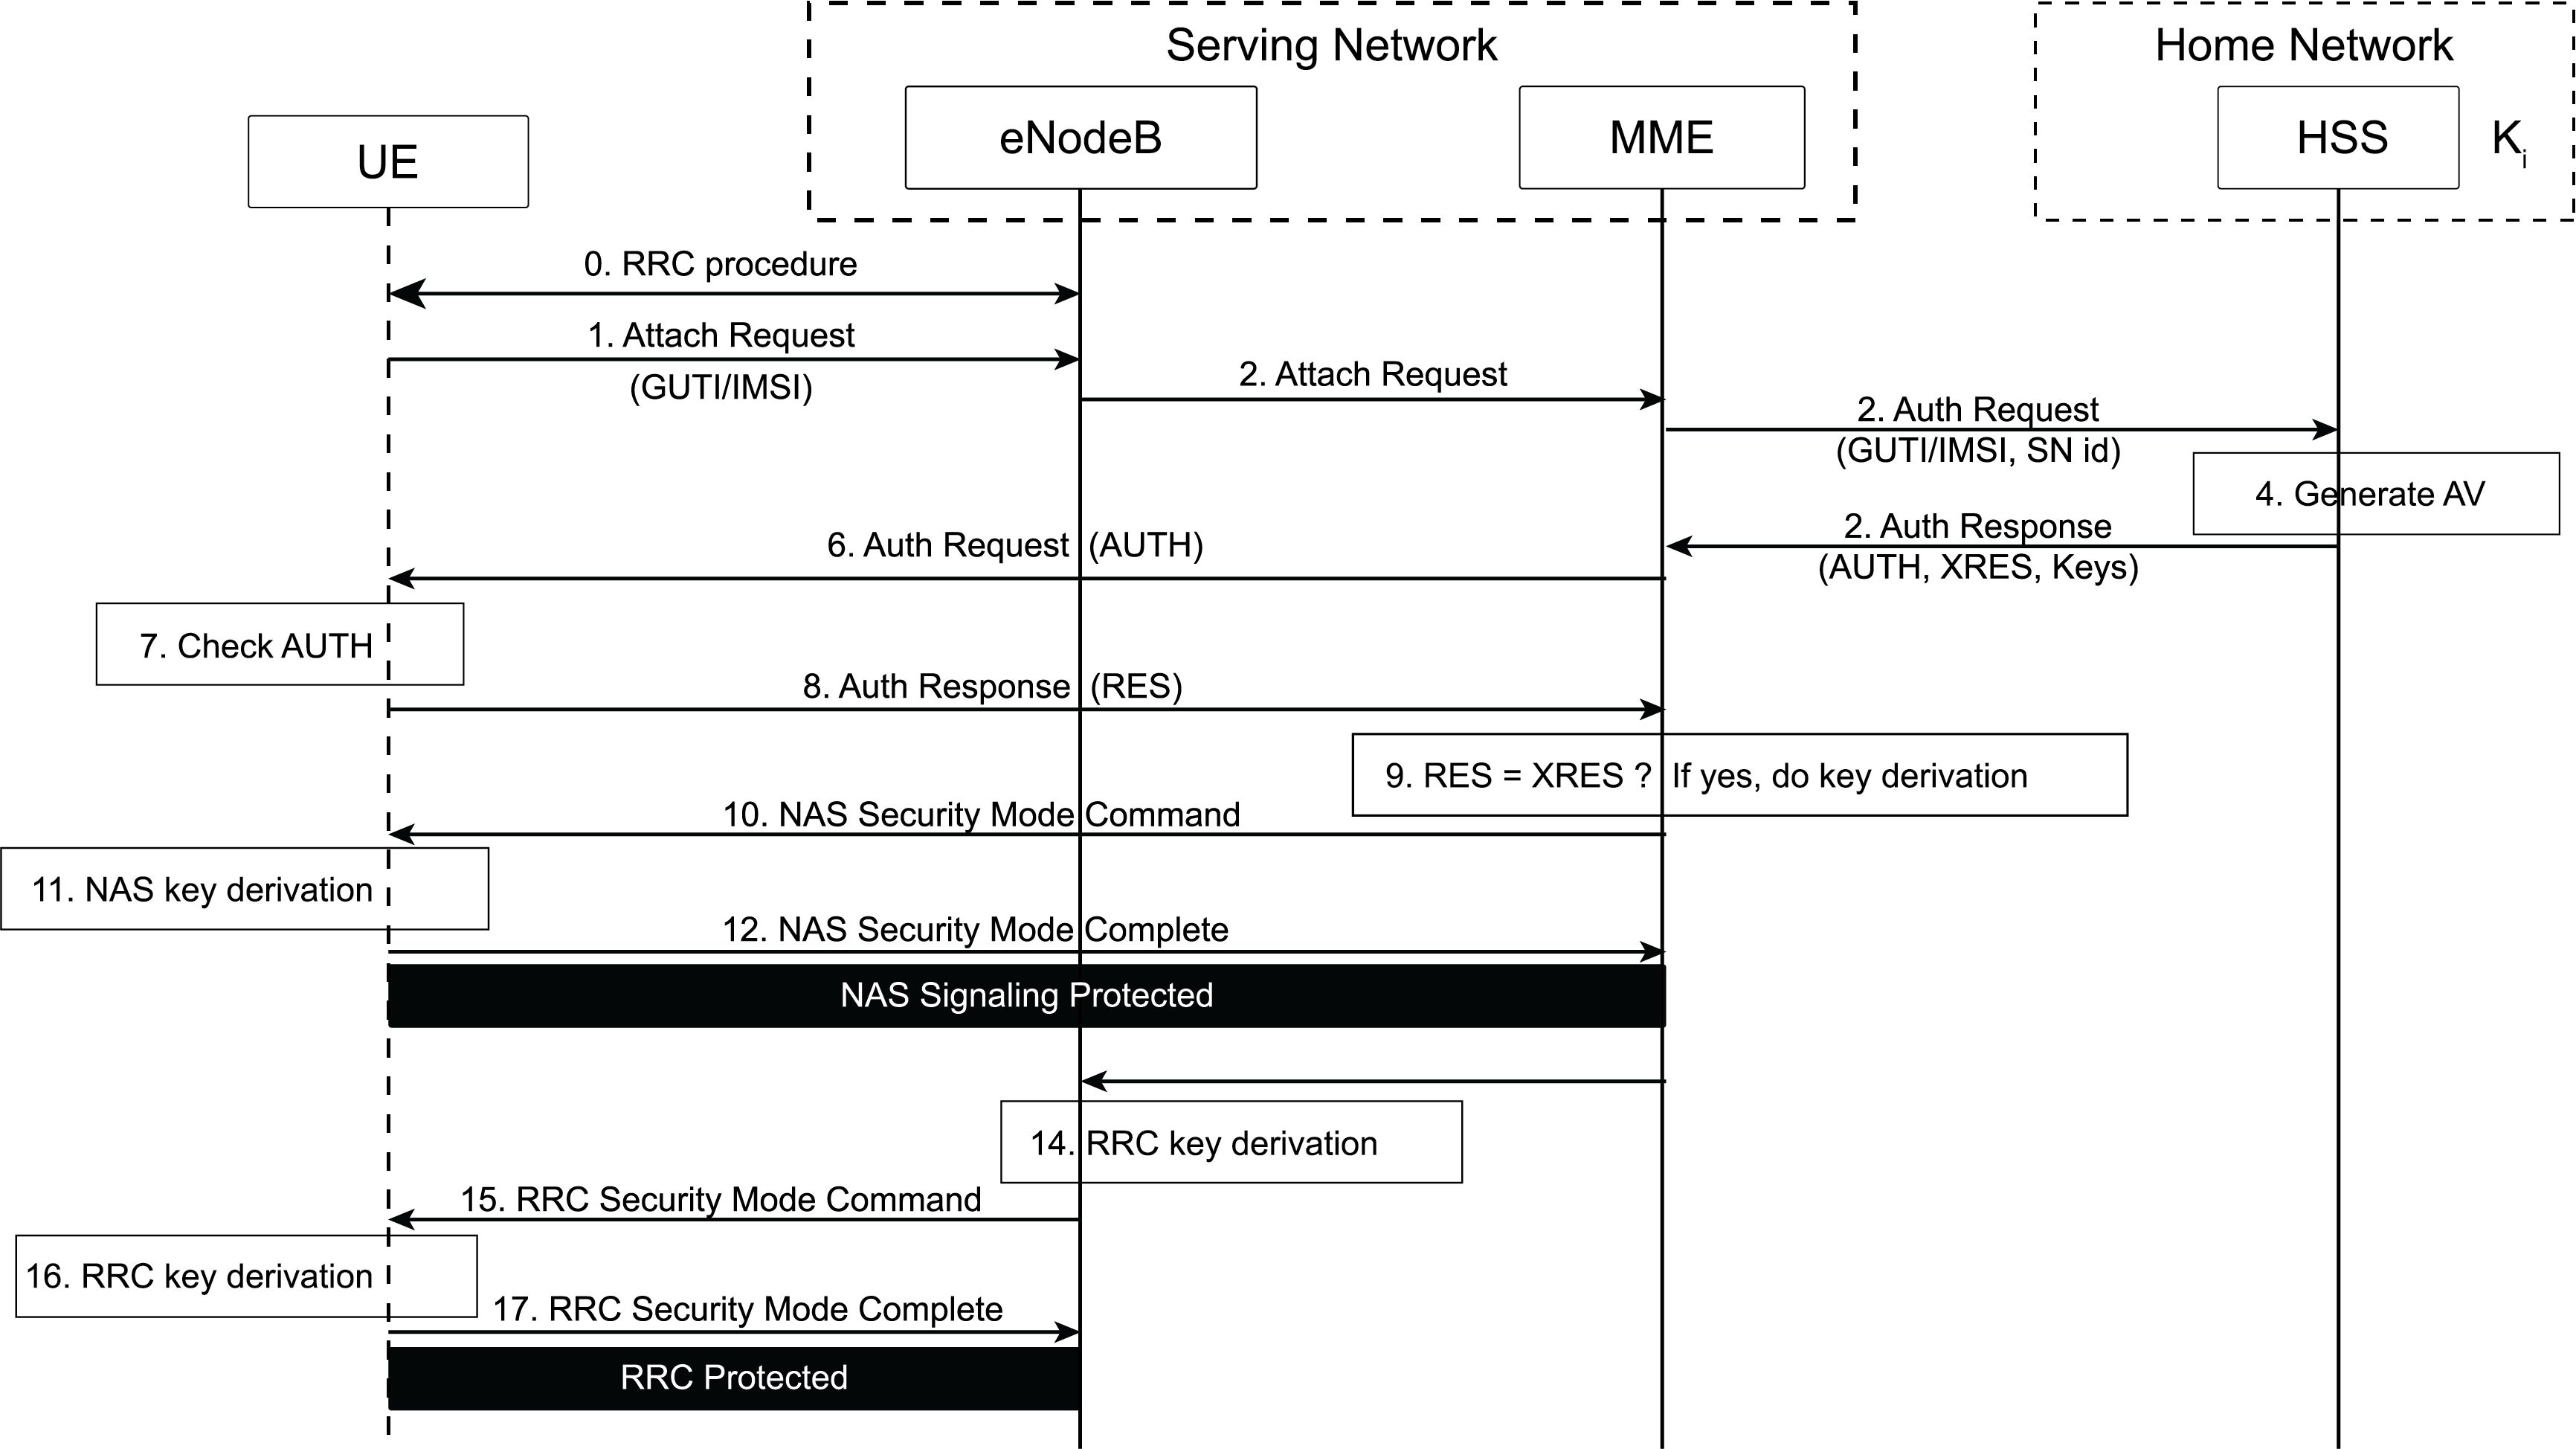
\includegraphics[width=0.8\textwidth]{figs/4g-authentication-flow.png}
    \caption{\ac{4G} Authentication Procedure}
    \label{fig:single}
\end{figure}

\subsection{\acs{5G} Security Framework}

As mentioned before, \ac{5G} has a \acl{SBA}, and in this architecture, some of the new entities relevant to \ac{5G} authentication are:

\begin{itemize}
    \item{
        The \ac{SEAF}, which acts as a intermidiary between the \ac{UE} and its home network, during the authentication process. It has the capability to out right reject and \ac{UE} but is dependent on the \ac{HN} to validate the authentication.
    }
    \item{
        The \ac{AUSF} is responsible to deciding if the \ac{UE} get authenticated.
    }
    \item{
        The \ac{UDM} hosts the \ac{ARPF}, responsible for selecting the authentication method, based on the subscribet identity and configured policy. It will also compute the authentication data for \ac{AUSF}.
    }
    \item{
        The \ac{SIDF} will be responsible for obtaining the \ac{SUPI} by decrypting the \ac{SUCI}.
    }
\end{itemize}

One of the main goals for \ac{5G} was the unification of authentication by making it open and access-network agnostic. In order to make it open, \ac{5G} rellies havily on \ac{EAP}, and when used the authentication will take place between the \ac{UE}, acting as the supplicant, the \ac{AUSF}, acting has the authenticaion server, through the \ac{SEAF} acting as an authenticator~\cite{rfc3748}.

Each generation of cellular networks has defined at least one new authentication method. For example, \ac{4G} introduced \ac{EPS-AKA}, and \ac{5G} introduced three authentication methods: \ac{5G-AKA}, \ac{EAP-AKA'}, and \ac{EAP-TLS}.

\subsection{Comparing \acs{5G-AKA}, \ac{EAP-AKA'} and \ac{EAP-TLS}}

The process begins when the \ac{SEAF} initiates authentication after receiving a message from the \ac{UE}. The \ac{UE} provides either a \ac{5G-GUTI} or a \ac{SUCI}.

The \ac{AUSF} first verifies that the requesting network is authorized. It then sends an authentication request to \ac{UDM}/\ac{ARPF}. If the \ac{SUCI} is provided, it's decrypted by the \ac{SIDF} to retrieve the \ac{SUPI}, which is then used to select the authentication method. \ac{UDM}/\ac{ARPF} generates an authentication response that includes tokens and keys, which are used by the \ac{AUSF} to compute a hash (\ac{HXRES}) and verify the expected response.

The \ac{AUSF} sends the authentication response to the \ac{SEAF} with the \ac{AUTH} token and \ac{HXRES}. At this point, the \ac{SUPI} is still not shared with the \ac{SEAF}. The \ac{SEAF} then forwards the \ac{AUTH} token to the \ac{UE}, which validates it using a secret key shared with the home network. If successful, the \ac{UE} computes and sends a response (\ac{RES} token) back to the \ac{SEAF}. The \ac{SEAF} validates this and forwards it to the \ac{AUSF} for final validation.

Once the \ac{RES} token is verified by the \ac{AUSF}, it sends an anchor key to the \ac{SEAF}, which then derives an \ac{AMF} key. The \ac{AMF} uses this key to generate further keys for protecting signaling messages between the \ac{UE} and the network elements. The \ac{UE}, with its root key, can derive all necessary keys for secure communication with the network, ensuring a shared and secure set of keys between the \ac{UE} and the network.

\ac{EAP-AKA'} is an alternative authentication method in \ac{5G}, providing mutual authentication between the \ac{UE} and the network based on a shared cryptographic key. Like \ac{5G-AKA}, it ensures strong security properties but has different message flows since it is based on \ac{EAP}. In this method, \ac{EAP} messages are encapsulated in \ac{NAS} messages between the \ac{UE} and the \ac{SEAF}, and in \ac{5G} service messages between the \ac{SEAF} and the \ac{AUSF}. In \ac{EAP-AKA'}, the \ac{SEAF} acts as a transparent relay, forwarding \ac{EAP} messages between the \ac{UE} and the \ac{AUSF} without participating in authentication decisions. In contrast, in \ac{5G-AKA}, the \ac{SEAF} verifies the \ac{UE}'s authentication response and can act on failures. Also, in 5G-AKA, the \ac{KAUSF} is computed by \ac{UDM}/\ac{ARPF} and sent to the \ac{AUSF} while in \ac{EAP-AKA'}, the \ac{AUSF} derives the \ac{KAUSF} from keying materials provided by the \ac{UDM}/\ac{ARPF}, using an \ac{EMSK} as specified in \ac{EAP}.

Lastly we have \ac{EAP-TLS} which is a subscriber authentication method in \ac{5G}, designed for specific scenarios like private networks and \ac{IoT}. When selected by \ac{UDM}/\ac{ARPF}, \ac{EAP-TLS} operates between the \ac{UE} and the \ac{AUSF} through the \ac{SEAF}, which acts as a transparent \ac{EAP} authenticator, forwarding \ac{EAP-TLS} messages. With \ac{EAP-TLS} we still achieve mutual authenticaion, this time via verification of public key certificates or a pre-shared key (\ac{PSK}) established through \ac{TLS} handshakes or out-of-band methods.

Some fundamental differences between this method and the previous AKA-based ones include the trust model: in \ac{EAP-TLS}, mutual trust is based on public key certificates, unlike AKA methods, which rely on symmetric keys shared between the \ac{UE} and the network. Additionally, \ac{EAP-TLS} eliminates the need to store numerous long-term symmetric keys in the home network (\ac{UDM}), reducing risks in key management. Another key difference that makes \ac{EAP-TLS} extremely well-suited for our use case is that it does not require the \ac{UE} to have a \ac{USIM}~\cite{cbl-comp-4g-5g-p12}.

\subsection{What is \ac{3GPP} and non-\ac{3GPP} access?}

ac{3GPP} encompasses standards for mobile networks like \ac{3G}, \ac{4G}, and \ac{5G}, which are cellular technologies enabling network services from mobile carriers. In contrast, non-\ac{3GPP} refers to access technologies not standardized by \ac{3GPP}, such as Wi-Fi or satellite networks, which can still integrate with \ac{3GPP} networks but follow different standards (e.g., IEEE for Wi-Fi).

Within \ac{3GPP} architecture, the terms trusted and untrusted define how non-\ac{3GPP} networks connect to the mobile core. Trusted networks are verified and approved by the mobile operator, connecting directly to the core network using secure protocols, similar to \ac{3GPP} networks. For instance, a mobile operator’s managed Wi-Fi network may be trusted. On the other hand, untrusted networks, like public Wi-Fi hotspots managed by third parties, do not meet these standards and are treated differently.

\section{Wi-Fi Integration Challenges}

\section{Authentication and Identity Management in \acs{5G}}

% subsection:
%   - What is a GUTI, SUPI, SUCI and NAI?

\section{Current Solutions and Proposals}
\include{chapters/architecture-and-implementation}
\chapter{Validation and Evaluation}%
\label{chapter:validation-and-evaluation}

\begin{introduction}
This chapter will describe our experimental setup, define the performance metrics used, and present the results of our solution's implementation. We'll analyze these results and compare our approach with existing solutions to demonstrate its effectiveness.
\end{introduction}
\chapter{Conclusion and Future Work}%
\label{chapter:conclusion-and-future-work}

\begin{introduction}
The final chapter will summarize our key contributions, discuss any limitations of our study, and provide recommendations for future research in this area. We'll reflect on how our work advances the field of 5G and Wi-Fi integration and suggest potential avenues for further investigation.
\end{introduction}

%%%%%%%%%%%%%%%%%%%%%%%%%%%%%%%%%%%%%%%%%%%%%%%%%%%%%%%
% End of Thesis text 
%%%%%%%%%%%%%%%%%%%%%%%%%%%%%%%%%%%%%%%%%%%%%%%%%%%%%%%

\backmatter

%%%%%%%%%%%%%%%%%%%%%%%%%%%%%%%%%%%%%%%%%%%%%%%%%%%%%%%
% Print all used references
%%%%%%%%%%%%%%%%%%%%%%%%%%%%%%%%%%%%%%%%%%%%%%%%%%%%%%%

\begingroup
\renewcommand{\bibfont}{\footnotesize}
% Redefine References name to Portuguese
% Change if you are using english
\defbibheading{bibliography}[References]{
  \chapter{#1}
}
\SingleSpacing
\setlength\bibitemsep{8pt}
\printbibliography[heading=bibliography]
\endgroup


%%%%%%%%%%%%%%%%%%%%%%%%%%%%%%%%%%%%%%%%%%%%%%%%%%%%%%%
% Load appendix
%%%%%%%%%%%%%%%%%%%%%%%%%%%%%%%%%%%%%%%%%%%%%%%%%%%%%%%

\mainmatterWithoutReset
\appendix

\chapter{Additional content}


\end{document}
